% Slides for 2024-07-02
% To create a slide, use the following:
% \begin{frame}{TITLE}
%     BODY
% \end{frame}

% To create a slide with a bullet list, use the following:
% \begin{frame}{TITLE}
%     \begin{itemize}
%         \item ITEM 1
%         \item ITEM 2
%     \end{itemize}    
% \end{frame}

% To create a slide with numbered list, use the following:
% \begin{frame}{TITLE}
%     \begin{enumerate}
%         \item ITEM 1
%         \item ITEM 2
%     \end{enumerate}
% \end{frame}

\begin{frame}{Project Overview for Summer}
    \begin{enumerate}
        \item Recall from last week.
    \end{enumerate}
    \centering
    \includegraphics[height=0.7\textheight,width=0.7\textwidth,keepaspectratio]{images/bom/oldslide.png}
\end{frame}

\begin{frame}{What is Done?}
    \centering
    \includegraphics[height=0.7\textheight,width=0.7\textwidth,keepaspectratio]{images/bom/oldslide.png}
\end

\begin{frame}{Troubles with LRMC...}
    \begin{enumerate}
        \item Really complex but publicily available!
        \item Written in MatLab... MatLab sucks with CLI...
        \item Octave is an alternate but no parrallel!
        \item Really need parrallel...
    \end{enumerate}
    \centering
    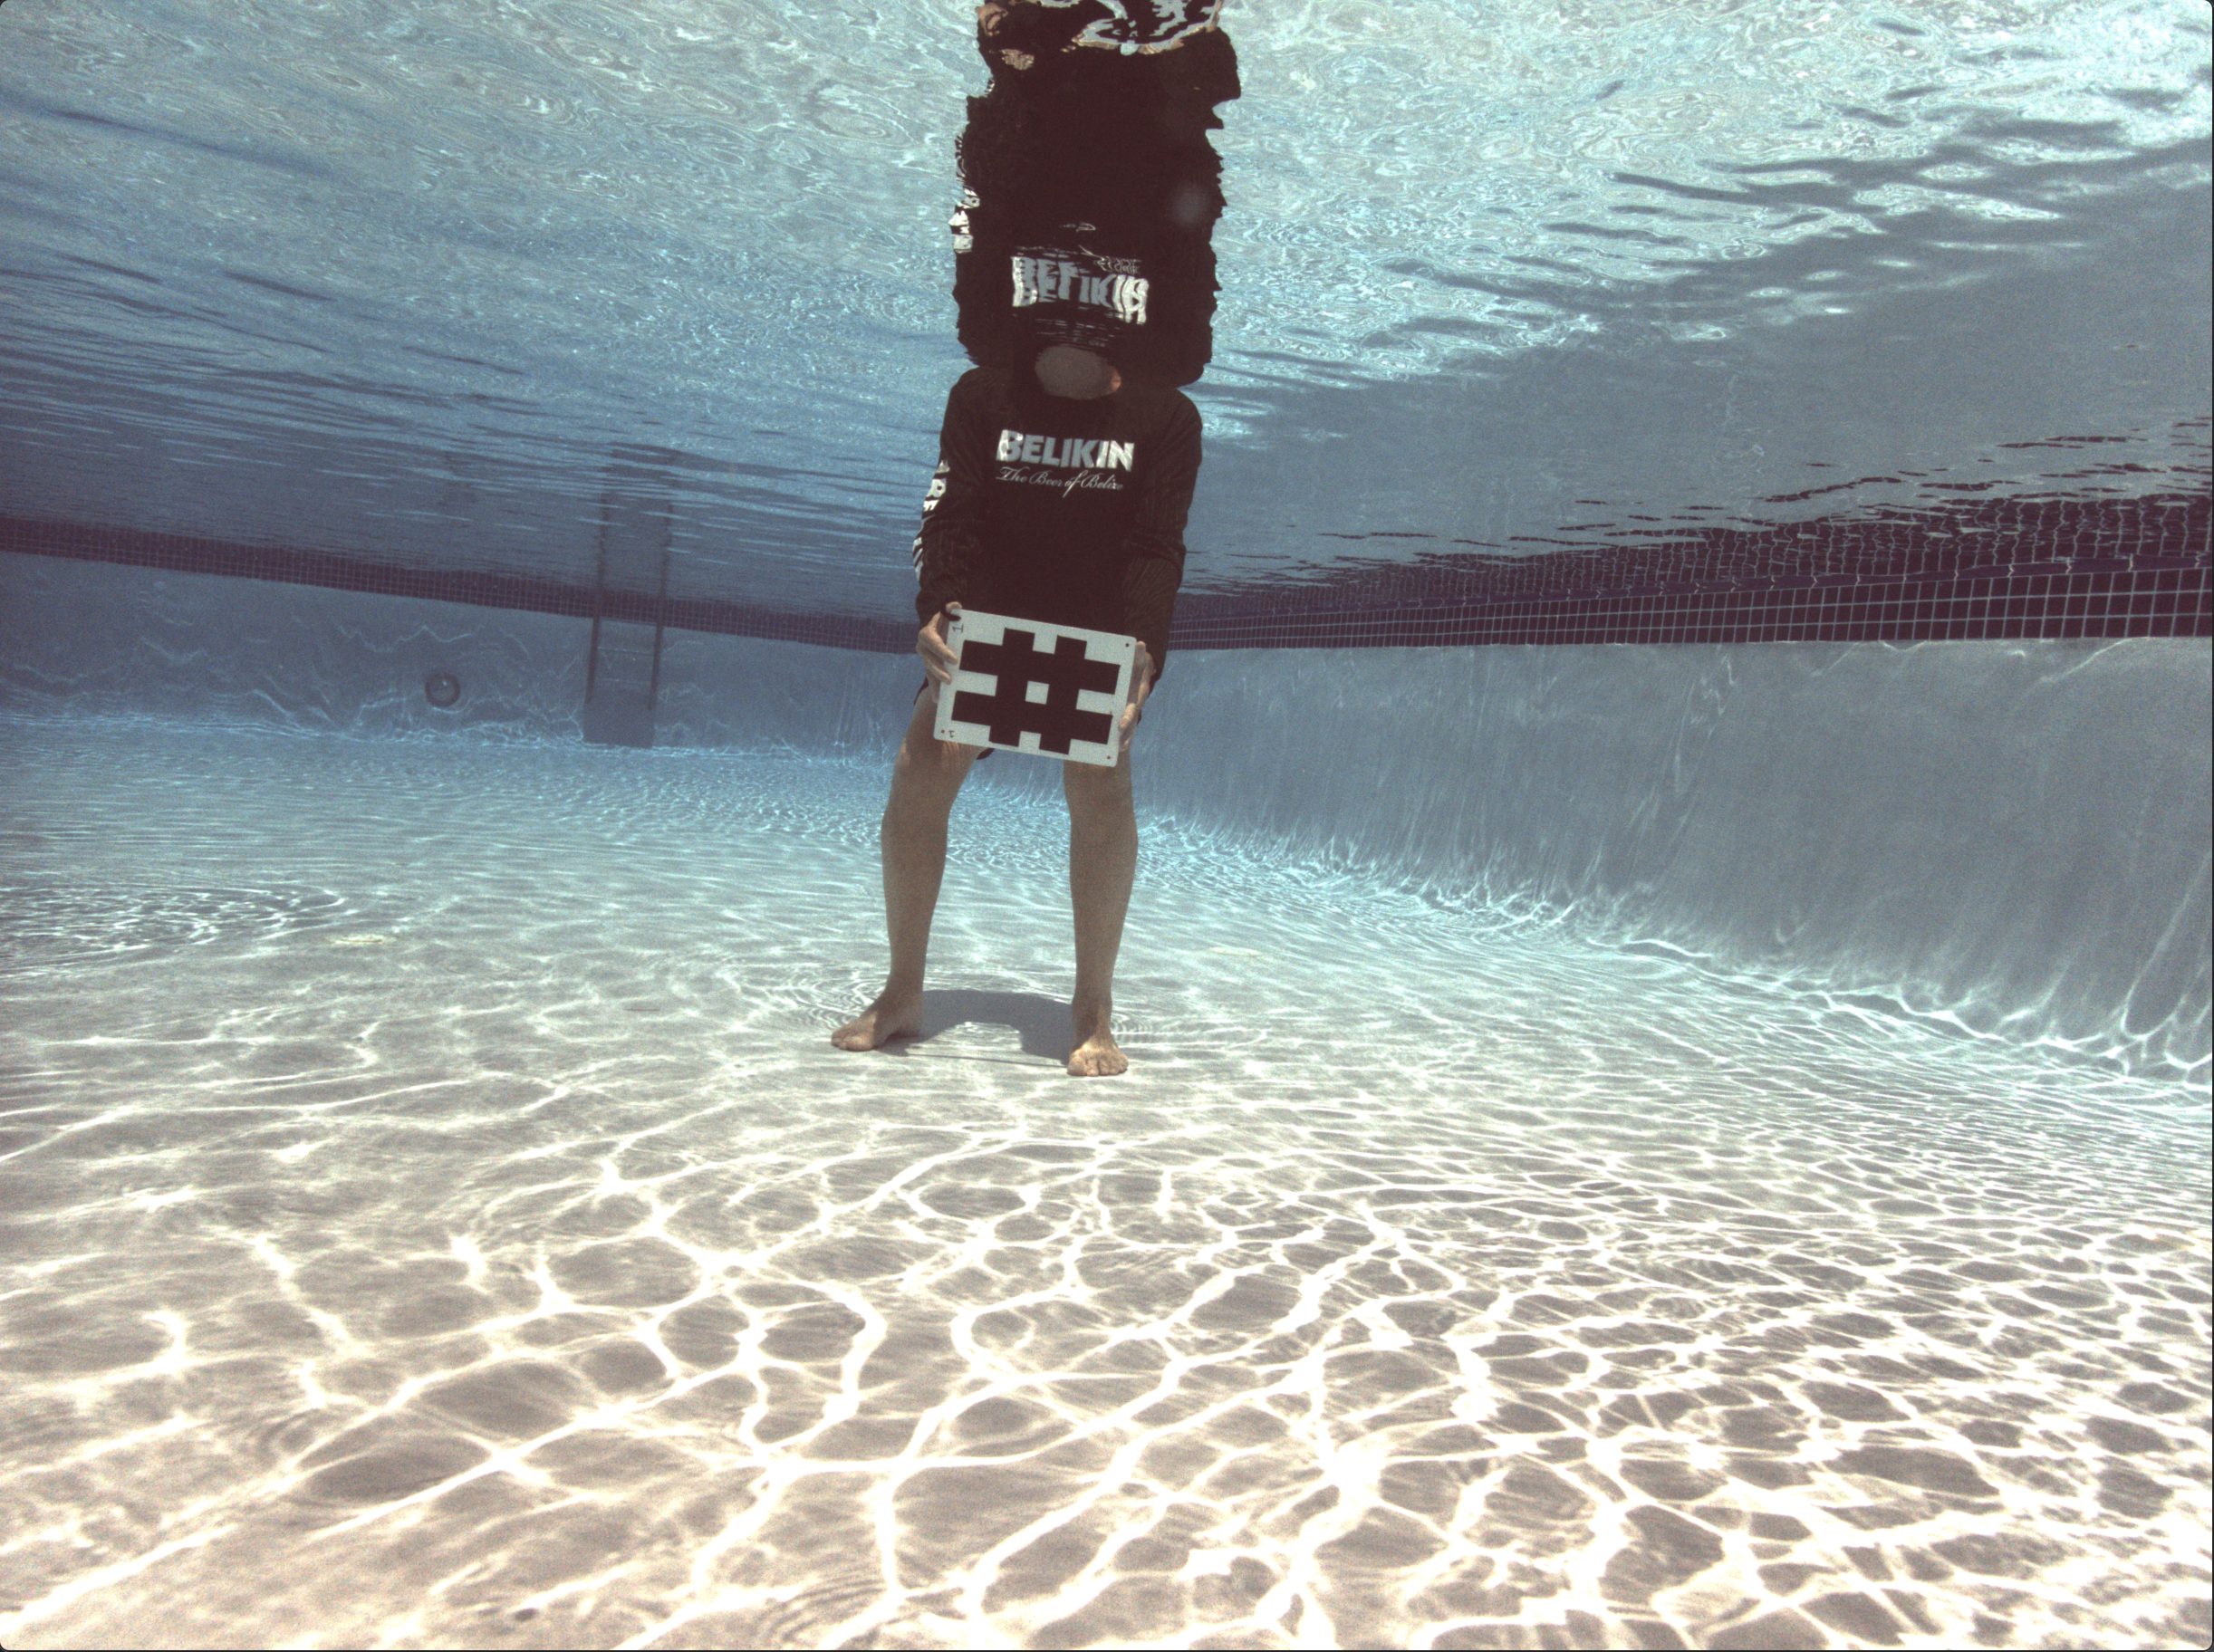
\includegraphics[height=0.7\textheight,width=0.7\textwidth,keepaspectratio]{images/bom/image.png}
\end

\begin{frame}{More Complication}
    \begin{enumerate}
        \item MatLab has an AWS deployment option
        \item Expensive and only MatLab GUI (maybe)
        \item Need Python for Sherlock
        \item For now MatLab on Kastner-ML?
    \end{enumerate}
    \centering
    \includegraphics[height=0.7\textheight,width=0.7\textwidth,keepaspectratio]{images/bom/matlab.png}
\end

\begin{frame}{Labeling}
    \centering
    \includegraphics[height=0.7\textheight,width=0.7\textwidth,keepaspectratio]{images/bom/labeling.png}
\end

% To create a slide with two columns, use the following:
% \begin{frame}{TITLE}
%     \begin{columns}
%         \begin{column}{0.5\textwidth}
%             COLUMN 1 BODY
%         \end{column}
%         \begin{column}{0.5\textwidth}
%             COLUMN 2 BODY
%         \end{column}
%     \end{columns}
% \end{frame}
